\documentclass[11pt]{article}
\usepackage{amsmath,amstext,amsfonts,amssymb,amsthm,epsfig,epstopdf,url,array}
\usepackage[margin=1in]{geometry}
\usepackage{xcolor}
\usepackage{graphicx}
\usepackage{times}

\theoremstyle{plain}
\newtheorem{thm}{Theorem}[section]
\newtheorem{lem}[thm]{Lemma}
\newtheorem{prop}[thm]{Proposition}
\newtheorem{cor}[thm]{Corollary}
\newtheorem{defn}[thm]{Definition}
\newtheorem{claim}[thm]{Claim}

\theoremstyle{definition}
\newtheorem{con}{Conjecture}[section]
\newtheorem{exa}{Example}[section]
\newtheorem*{sol}{Solution}
\newtheorem{cdef}{Definition}[section]


\theoremstyle{remark}
\newtheorem{rem}{\textbf{Remark}}
\newtheorem*{note}{\color{blue}\textbf{Note}}
\usepackage{qtree}


\usepackage{hyperref}

\usepackage[nameinlink,noabbrev,capitalize]{cleveref} 
\crefalias{subequation}{equation}
\crefalias{thm}{theorem}


% to make cleveref print ``Lemma'' for lemma
\let\oldlemma\lem
\renewcommand{\lem}{%
  \crefalias{thm}{lem}% Theorem counter now looks like Lemma
  \oldlemma}
\Crefname{lem}{Lemma}{Lemmas}

% to make cleveref print ``Definition for definition
\let\olddefn\defn
\renewcommand{\defn}{%
  \crefalias{thm}{defn}% Theorem counter now looks like Definition
  \olddefn}
\Crefname{defn}{Definition}{Definitions}

% to make cleveref print ``Remark for remark
\let\oldrem\rem
\renewcommand{\rem}{%
  \crefalias{thm}{rem}% Theorem counter now looks like Remark
  \oldrem}
\Crefname{rem}{Remark}{Remarks}

% to make cleveref print ``Corollary for corollary
\let\oldcor\cor
\renewcommand{\cor}{%
  \crefalias{thm}{cor}% Theorem counter now looks like Corollary
  \oldcor}
\Crefname{cor}{Corollary}{Corollaries}

% to make cleveref print ``Claim for claim
\let\oldclaim\claim
\renewcommand{\claim}{%
  \crefalias{thm}{claim}% Theorem counter now looks like Claim
  \oldclaim}
\Crefname{claim}{Claim}{Claims}

% to make cleveref print ``Proposition for prop
\let\oldprop\prop
\renewcommand{\prop}{%
  \crefalias{thm}{prop}% Theorem counter now looks like Prop
  \oldprop}
\Crefname{prop}{Proposition}{Propositions}

% to make cleveref print ``Conjecture for conj
\let\oldcon\con
\renewcommand{\con}{%
  \crefalias{thm}{con}% Theorem counter now looks like Con
  \oldcon}
\Crefname{con}{Conjecture}{Conjectures}

% Editing commands requiring color package
\newcommand{\add}[1]{\textcolor{blue}{#1}}
\newcommand{\delete}[1]{\textcolor{red}{#1}}
\definecolor{darkgrn}{rgb}{0, 0.8, 0}
\newcommand{\modified}[1]{\textcolor{darkgrn}{#1}}

\newcommand{\txbl}[1]{\textcolor{blue}{#1}}
\newcommand{\txrd}[1]{\textcolor{red}{#1}}
\newcommand{\txgr}[1]{\textcolor{green}{#1}}
\newcommand{\txcr}[1]{\textcolor{crimson}{#1}}


% shortcut commands
\newcommand{\sym}[1]{\mathcal{S}^{#1}}

\title{Robust Feasibility of Systems of Quadratic Equations Using Topological Degree Theory}

\author{Krishnamurthy Dvijotham\thanks{\affil{Google DeepMind}}
    \hspace*{0.3in}
  Bala~Krishnamoorthy\thanks{\affil{Washington State University}}
  \hspace*{0.3in}
  Benjamin Rapone\footnotemark[2]
}


\bibliographystyle{plain}

\begin{document}

\maketitle

\begin{abstract}
  We consider the problem of measuring the \emph{margin of robust feasibility} of solutions to a system of nonlinear equations.
%  \txgr{Define robustness margin informally here... }\\
  This problem turns out to be NP-hard in general.
  We study the special case of a system of quadratic equations, which shows up in many practical applications such as the power grid and other infrastructure networks. 
  We develop approaches based on topological degree theory to estimate bounds on the robustness margin of such systems.
  Our methods use tools from convex analysis and optimization theory to cast the problems of checking the conditions for robust feasibility as a nonlinear optimization problem.
  We then develop \emph{inner bound} and \emph{outer bound} formulations for this optimization problem, which could be solved efficiently to derive lower and upper bounds, respectively, for the margin of robust feasibility.
  We evaluate our approach numerically on standard instances taken from the MATPOWER database of AC power flow equations that describe the steady state of the power grid.
  The results demonstrate that our approach can produce tight lower and upper bounds on the radius of robust feasibility for such instances.
\end{abstract}



\section{Introduction}
  This paper studies quadratic systems of equations with parameters.
  More concretely, we study a system of $n$ quadratic equations $F(\bold x)=\bold u$ where $F: \mathbb{R}^n \mapsto \mathbb{R}^n,\bold  x,\bold u \in \mathbb{R}^n$ and $F$ is quadratic in $\bold x$.
  We are interested in situations where the parameters $\bold u$ are uncertain and we are still interested in guaranteeing that there is a solution to $F(\bold x) = \bold u$ for $\bold x$ within limits on $\bold x$ and $\bold u$.
  Questions of this type arise in a variety of applications from analysis of stochastic processes to infrastructure networks like the power grid and the gas grid.
  For example, in binary markov trees, the parameter $\bold u$ represents the initial probabilities of the Markov chain.
  
Robust feasibility and optimization have been well-studied by both the optimization and topology communities. 
What is lacking is an approach that can gaurantee and quantify robust feasibility on large scale systems in an efficient manner. 
In this article we address this deficiency by developing theory that utilizes results from topological degree theory and convex optimization. 
We provide a theoretical foundation for determining robust feasibility of systems of quadratic equations and computational methods for producing lower and upper bounds on the maximum error bound for which one can guarantee robust solvability (the radius of robust solvability). 
To highlight the efficacy of our approach we derive models, which we test numerically on several quadratic systems constructed from the AC power flow equations that describe the steady state of the power grid with added uncertainty. 
The results show that our approach can be applied to large scale systems to produce tight lower and upper bounds on the radius of robust solvability, which we shall define as the robustness margin of the system.

In optimization, the focus has been on robust \emph{convex} optimization where uncertainty sets are specified for the parameters of a convex optimization problem (typically an LP or conic program) \cite{ben2009robust}.
Robust \emph{nonconvex} optimization has received only limited attention (a notable exception is the work of Bertsimas et al.~\cite{BeNoTe2010}).
These approaches {\em do not provide rigorous guarantees for robust feasibility with nonconvex constraints}.

In algebraic topology, there have been a number of studies on these problems based on several approaches, including ones based on robustness of level sets and persistent homology \cite{BeEdMoPa2010,EdMoPa2011}, well groups and diagrams \cite{ChSkPa2012,FrKr2016well,FrKr2016pers}, topological degree and robust satisfiability \cite{FrKr2015,FrKrWa2016},  and on Borsuk's theorem and interval arithmetic \cite{FrRa2015,FrHoLa2007,FrLa2005}.
While the theory developed by these approaches is fairly complete, the associated algorithms typically rely on explicit simplicial or cellular decompositions of the problem space.
But the size of such decompositions typically grows exponentially in the problem dimension, and hence these \emph{algorithms are typically impractical for large-scale applications}.

Looking specifically at applications such as the power systems, there has been significant interest in solving the non-robust version of the OPF problem to global optimality.
The driver has been the development of strong convex relaxations of the nonconvex optimization problems combined with ideas from global optimization such as spatial branch-and-cut, bound tightening, etc.~\cite{BiMu2016,coffrin2015strengthening}.
Uncertainty has been handled in a chance-constrained framework \cite{BiChHa2014,zhang2011chance}.
However, this approach has typically been applied only to linear approximations or convex relaxations of the AC power flow equations, and \emph{does not guarantee feasibility with respect to the true nonlinear power flow equations} \cite{BiChHa2014,kocuk2016strong,RoVrOlAn2015,TsBiTa2016}.


\section{Problem formulation}

%\delete{no need to specify these as a list... only uncommon notation appears to be that of $\sym{n}$. Could introduce only the required new notation in a paragraph.}
%\begin{itemize}
%\item[] $\mathbb{R}$: Set of real numbers, $\mathbb{R}^n$: $n$-dimensional Euclidean space 
%\item[] $\modified{\sym{n}}$: Set of $n \times n$ symmetric matrices \delete{$\mathbb{S}$ is often used to denote other spaces.}
%\item[] $\mathbb{R}^{n \times m}$: Set of $n \times m$ real matrices
%\item[] $x \in \mathbb{R}^n$: $x$ is a real vector variable
%\item[] $M \geq 0$ (for $M \in \mathbb{R}^{n \times n}$): $M$ is a matrix with all entries non-negative  
%\item[] $A \in \mathbb{R}^{n\times n}$: $A$ is a potentially sparse condition matrix
%\item[] $b \in \mathbb{R}^n$: $b$ is a non-zero vector with all components non-negative
%\end{itemize}

We study systems of quadratic equations of the form
\begin{align}
& Q(\bold x)+L\bold x=\bold u\label{eq:Quad}
\end{align}
where $Q: \mathbb{R}^n \mapsto \mathbb{R}^n$ is a vector-valued quadratic function, that is, there exist symmetric matrices $\mathcal{M}^1,\ldots,\mathcal{M}^{n} \in \sym{n}$, ($\sym{n}$ the set of $n \times n$ symmetric matrices) such that
\[[Q(\bold x)]_i = \bold x^t \mathcal{M}_{i} \bold x \quad \forall i \in [n]\]
and $L \in \mathbb{R}^{n\times n}$, $\bold u \in \mathbb{R}^n$. 
We are interested in solutions to this system of equations under linear constraints of the form
\begin{align}
(A\bold x)_i\leq b_i \quad \forall i \in [n]\label{eq:xLimits}
\end{align}
However, the parameter $\bold u$ is uncertain and only known upto certain error bounds
\begin{align}
u^{\min}_i=u_i^*-e_i \leq u_i \leq =u_i^*+e_i=u^{\max}_i \quad \forall i \in [n] \label{eq:uLimits}
\end{align}
where $\bold u^*$ is a forecast for $\bold u$ and $\bold e$ denotes the error bounds associated with the forecast. 
For example, in the case of quadratic equations appearing in infrastructure networks like the power grid, $u_i$ represents uncertain power generation or consumption (for example uncertain weather-dependent power sources like solar or wind power). 
In the case of stochastic processes, $\bold u^*$ represents an initial state distribution.

\begin{figure}
\begin{center}
\includegraphics[scale=0.5]{Figures/Rfeas}
\end{center}
\caption{Robust Feasibility}
\label{fig:RFeas}
\end{figure}

\begin{cdef}[Robust Feasibility and Robust Margin problem]
\label{RobustDef}
Determine whether for all values of $\bold u$ satisfying \eqref{eq:uLimits}, the system of equations \eqref{eq:Quad} has a solution for $\bold x$ satisfying the constraints \eqref{eq:xLimits}. 
If this is true, the system \eqref{eq:Quad},\eqref{eq:xLimits},\eqref{eq:uLimits} is said to be \emph{robust feasible}. 
The largest $r$ s.t. $e_i\geq r \ \forall i \ s.t. \ e_i>0$ in \eqref{eq:uLimits} s.t. the system \eqref{eq:Quad},\eqref{eq:xLimits},\eqref{eq:uLimits} is robust feasible is said to be the \emph{robustness margin}. 
See \cref{fig:RFeas} for a pictorial depiction. 
\end{cdef}

The definition for robustness margin is left here in its most general form so as to capture all scenarios under which a researcher may find themselves. 
For instance it very well may be the case that only some of the dimensions of $\bold u$ will have margins of uncertainty. 
Furthermore, one may have need of computing the robustness margin for only a subset of the dimensions of $\bold u$ which pertain to problem areas or nodes of particular interest to the research. 
This manual restriction will of course produce a robustness margin greater than or equal to that obtained by considering all dimensions, which certainly remains an option under the current setting. 

\section{Theoretical results}
We now describe the main technical results of this paper. 
In the first subsection we describe the setting under which the problem can be solved using the results which follow. Our results take advantage of the well studied area of topological degree theory. 
For an introduction to topological degree theory see \cite{OrChCh2006}, \cite{fonseca1995degree} and \cite{MoVrYa2002}. 
Suffice it then to say that should $\Omega\subset\mathbb{R}^{n}$ be open and bounded, $F:\Omega\rightarrow \mathbb{R}$ continuous, and $F(\bold x)\neq \bold y \quad \forall \bold x\in\partial\Omega$ for some $\bold y\in\mathbb{R}^n$, then the degree of $F$ at $y$ over $\Omega$, denoted $d\left(\Omega,F,\bold y\right)\in\mathbb{Z}$, is defined. 
For the purposes of this article we utilize the following property for the degree as our definition of the topological degree of a function $F$ at $y$ over a set $\Omega$. 
See \cite{OrChCh2006} for details.:
\begin{equation}\label{eq:Deg3}
d\left(f,\Omega,\bold y\right)=\sum\limits_{\bold x\in f^{-1}(\bold y)}\operatorname{sign}\left(J_f(\bold x)\right)
\end{equation}

Where $\operatorname{sign}\left(J_f(\bold x)\right)$ denotes the sign of the Jacobian of $F$ at $\bold x$, i.e.:

\[\operatorname{sign}\left(J_f(\bold x)\right)=   \left\{
\begin{array}{ll}
       \ -1   & \mbox{if } J_f(\bold x)< 0, \\
      \quad 0 & \mbox{if } J_f(\bold x)= 0,~\mbox{ and } \\
      \quad 1 & \mbox{if } J_f(\bold x)> 0. \\
\end{array} 
\right. \]

Additionally we utilize the following two common properties of the topological degree. 
See \cite{OrChCh2006} for details. \\
If $H : [0,1]\times\bar{\Omega}\rightarrow\mathbb{R}^n$ is continuous such that $H(t,\bold x)\neq \bold y \quad \forall t\in[0,1]\quad \bold x\in\partial\Omega$,   \ then 
\begin{equation}\label{eq:Deg1} 
d\left(\Omega,H(t,\cdot),\bold y\right)\text{ does not depend on }t.
\end{equation}

\begin{equation}\label{eq:Deg2}
\text{If }d(\Omega,F,\bold y)\neq 0,\text{ then there exists }\bold x\in\Omega\text{ s.t. }F(\bold x)=\bold y. 
\end{equation}


Let $F(\bold x)=Q(\bold x)+L(\bold x)$, $\Omega=\{\bold x| A\bold x< \bold b\}$ and $\hat{\bold x}\in Int(\Omega)$ be a solution to the forecasted system $F(\bold x)=\bold u^*$ in \ref{eq:Quad}, such that $\operatorname{sign}\left(J_{F}(\hat{\bold x})\right)\neq 0$ (for a review of efficient methods of verification see \cite{GRIEWANK2014}). 
If no solutions exist then certainly the system is not robust feasible. Define $\Omega_u=\{\bold u| \bold u\text{ satisfies }\ref{eq:uLimits}\}$.
Verify using existing methods or those adopted from this paper that no other solutions exist in $Int(\Omega)$ (this may require further restricting the domain or even a slight perturbation of the forcasted $\bold u$). 
Thus by \ref{eq:Deg2} and \ref{eq:Deg3} we have verified that $d\left(\Omega, F(\bold x), \bold u^*\right)\neq 0$. 
Note that this is not the only method for verification, but in some sense the easiest to carry out. \\

Let $L$ represent an arbitrary line passing through $\bold u^*$, and $\bold l_{min},\bold l_{max}$ the two points of intersection between $\partial\Omega_u$ and $L$. 
Define a homotopy $H_L : [0,1]\times\bar{\Omega}\rightarrow\mathbb{R}^n$ as 
\begin{align}
H_L(t,\bold x) = F(\bold x)-\left[(1-t)\bold l_{min}+t\bold l_{max}\right] \label{eq:Homo}
\end{align}

Observe that by construction $H_L\left(\frac{1}{2},\hat{\bold x}\right)=F(\hat{\bold x})-\bold u^*=\textbf{0}$. 
Thus if no other solutions to $H_L\left(\frac{1}{2},\bold x\right)=0$ exist in $\Omega$ and $\operatorname{sign}\left(J_{H_{L,\frac{1}{2}}}(\hat{\bold x})\right)\neq 0$ then we have that $d(\Omega,H_L\left(\frac{1}{2},\bold x\right),\textbf{0})\neq 0$ by \ref{eq:Deg3}. 
Since $L$ was arbitrary this holds for all such lines passing through $\bold u^*$.\\
Note that for each $\hat{\bold u}\in\Omega_u\setminus\{\bold u^*\}$, $\exists !$ $\hat{L}$ passing through $\bold u^*$ and $t\in[0,1]$,  s.t. $\hat{\bold u}=(1-t)\hat{\bold l}_{min}+t\hat{\bold l}_{max}$. 
Therefore if $d(\Omega,H_L\left(\frac{1}{2},\bold x\right),\bold 0)\neq 0$ for each choice of $L$, it follows by \ref{eq:Deg1} that the robust solvability problem can be determined by validating or invalidating the following statement:
\begin{align}
\not\exists \bold x\in\partial\Omega, \ s.t. \ F(\bold x)-\bold u=\bold 0	 \ \ for \ any \ \ \bold u\in\Omega_u. \label{eq:RSForm}
\end{align}

From here on we will assume $d(\Omega,H\left(\frac{1}{2},\bold x\right),\bold 0)\neq 0$ and focus our efforts on the development of methods for validating or invalidating \ref{eq:RSForm}.\\



\begin{lem} \ \\
\label{lem:BdOpt}
Let $X\subset\mathbb{R}^n$ be closed and $\bold{f}:\mathbb{R}^n\rightarrow\mathbb{R}^n$ be continuous. 
If $\bold{f}$ has no singularities and $$\min\limits_{||\bold{\lambda}||=1}\max\limits_{\bold x\in X}\ \bold{\lambda}^T\bold{f}(\bold x)$$
obtains its optimal at $\bold{\hat{x}}$,$\bold{\lambda}_{\bold{\hat{x}}}$ then $\bold{f}(\bold{\hat{x}})\in \partial \bold{f}(X)$. 

\begin{proof} \ \\
(By contradiction) Assume $\bold{f}(\bold{\hat{x}})\in \bold{f}(X)\setminus\partial \bold{f}(X)$. 
Let $\theta$ the angle between $\bold{\lambda}_{\bold{\hat{x}}}$ and $\bold{\hat{x}}$. 
Thus $\min\limits_{||\bold{\lambda}||=1}\max\limits_{x\in X}\ \bold{\lambda}^T\bold{f}(x)=\bold{\lambda}_{\bold{\hat{x}}}^T\bold{f}(\bold{\hat{x}})=|\bold{f}(\bold{\hat{x}})|\cos(\theta)$. 
Since $X\in\mathbb{R}^n$ is closed it is thus compact which implies $\bold{f}(X)$ is also compact. 
Thus $\exists r>0$ s.t. (ball of radius $r$ centered at $\bold{f}(\bold{\hat{x}})$) $B_r(\bold{f}(\bold{\hat{x}}))\in \bold{f}(X)\setminus\partial \bold{f}(X)$. 
Let $y$ be the antipodal point on $\partial B_r(\bold{f}(\bold{\hat{x}}))$ to the point of intersection between the line segment connecting the origin to $\bold{f}(\bold{\hat{x}})$ and $B_r(\bold{f}(\bold{\hat{x}}))$. 
It follows then that $|y|>|\bold{f}(\bold{\hat{x}})|$ and $\theta$ is the angle between $\bold{\lambda}_x$ and $y$.   
Let $\bold{x^*}\in X$ s.t. $\bold{f}(\bold{x^*})=y$, such a $\bold{x^*}$ exists as $\bold{f}(X)$ is compact. 
Therefore $\bold{\lambda}_{\bold{\hat{x}}}^T\bold{f}(\bold{x^*})=|\bold{f}(\bold{x^*})|\cos(\theta)>|\bold{f}(\bold{\hat{x}})|\cos(\theta)=\bold{\lambda}_{\bold{\hat{x}}}^T|\bold{f}(\bold{\hat{x}})|$ which is a contradiction. 
The lemma now follows.
\end{proof}
\end{lem}

\begin{thm} \ \\
\label{thm:MainIneq}
Let $X\subset\mathbb{R}^n$ be closed and $\bold{f}:\mathbb{R}^n\rightarrow\mathbb{R}^n$ be continuous s.t. $\bold{f}(X)$ contains the origin. 
If $\bold{f}$ has no singularities then $$\min\limits_{||\bold{\lambda}||=1}\max\limits_{\bold x\in X}\ \bold{\lambda}^T\bold{f}(\bold x)\geq \min\limits_{\bold x\in \partial X}\max\limits_{||\bold{\lambda}||=1}\ \bold{\lambda}^T\bold{f}(\bold x)$$
\begin{proof} \ \\
If the origin lies on the boundary of $\bold{f}(X)$ then let $\hat{\bold x}\in \partial X$ s.t. $f(\hat{\bold x})=\textbf{0}$. 
Such an $\hat{\bold x}$ exists as $f$ has no singularities. 
Then  clearly $$\min\limits_{||\bold{\lambda}||=1}\max\limits_{\bold x\in X}\ \bold{\lambda}^T\bold{f}(\bold x)\geq \min\limits_{||\bold{\lambda}||=1}\bold{\lambda}^T\bold{f}(\hat{\bold x})= 0 = \max\limits_{||\bold{\lambda}||=1}\ \bold{\lambda}^T\bold{f}(\hat{\bold x}) \geq \min\limits_{\bold x\in \partial X}\max\limits_{||\bold{\lambda}||=1}\ \bold{\lambda}^T\bold{f}(\bold x)$$
Thus assume the origin lies in the interior of $\bold{f}(X)$.
Let $\bold{\hat{x}}$ be the point and $\bold{\lambda}_{\bold{\hat{x}}}$ the unit vector at which $$\min\limits_{||\bold{\lambda}||=1}\max\limits_{\bold x\in X}\ \bold{\lambda}^T\bold{f}(\bold x)$$
obtains its optimal. \\

Case 1: If the angle, $\theta$, between $\bold{\hat{x}}$ and $\bold{\lambda}_{\bold{\hat{x}}}$ is 0 then $\max\limits_{||\bold{\lambda}||=1}\bold{\lambda}^T\bold{f}(\bold{\hat{x}})=\bold{\lambda}_{\bold{\hat{x}}}^T\bold{f}(\bold{\hat{x}})$. 
Furthermore by \cref{lem:BdOpt} $\bold{f}(\bold{\hat{x}})\in \partial \bold{f}(X)$ and thus $\bold{\hat{x}}\in \partial X$ since $\bold{f}$ has no singularities by hypothesis. 
It follows now that $$\min\limits_{\bold x\in \partial X}\max\limits_{||\bold{\lambda}||=1}\ \bold{\lambda}^T\bold{f}(\bold x)\leq \max\limits_{||\bold{\lambda}||=1}\ \bold{\lambda}^T\bold{f}(\hat{\bold x})=\bold{\lambda}_{\bold{\hat{x}}}^T\bold{f}(\bold{\hat{x}})=\min\limits_{||\bold{\lambda}||=1}\max\limits_{\bold x\in X}\ \bold{\lambda}^T\bold{f}(\bold x)$$

Case 2: Assume $\theta \neq 0$. 
Let $\bold{x^*}$ be a point on the boundary of $X$ s.t. the angle between $\bold{\lambda}_{\bold{\hat{x}}}$ and $\bold{f}(\bold{x^*})$ is 0. 
Such a point must exist as $\bold{f}(X)$ is compact and by hypothesis $\bold{f}(X)$ contains the origin, has no singularities ($\bold{f}$ maps $\partial X$ to $\partial \bold{f}(X)$) and by assumption the origin lies in the interior of $\bold{f}(X)$. 
It follows then that $$\min\limits_{\bold x\in \partial X}\max\limits_{||\bold{\lambda}||=1}\ \bold{\lambda}^T\bold{f}(\bold x)\leq \max\limits_{||\bold{\lambda}||=1}\bold{\lambda}^T \bold{f}(\bold{x^*}) =\bold{\lambda}_{\bold{\hat{x}}}^T\bold{f}(\bold{x^*})\leq \max\limits_{\bold x\in X}\bold{\lambda}_{\bold{\hat{x}}}^T\bold{f}(\bold x)=\min\limits_{||\bold{\lambda}||=1}\max\limits_{\bold x\in X}\ \bold{\lambda}^T\bold{f}(\bold x)$$

The theorem now follows.

\end{proof}
\end{thm}

\cref{thm:MainIneq} and \cref{lem:BdOpt} provide us with the theoretical tools we need to develop models for approximating the robustness margin.
We will use the terminology "inner bound models" to describe the process of verifying robust feasibility while expanding the uncertainty box centered at $\bold u*$ in order to compute the lower bounds on the robustness margin, which these models undertake. 
We use the terminology "outer bound models" to capture in a similar fashion the procedure used to compute the upper bounds on the robustness margin by contracting the uncertainty box until the system may be robust feasible. 
As such we dedicate the remainder of this section to the development of these inner and outer bound formulations. 

\subsection{Inner Bound Formulations}

\begin{thm}
Let $\Omega=\{\bold x| A\bold x< \bold b\}$, $\Omega_{u}=\{\bold u| u^{\min}_i\leq u_i \leq u^{\max}_i \ \forall i \}$, and $F(\bold x)=Q(\bold x)+L(\bold x)$ as described in \eqref{eq:Quad}, \eqref{eq:xLimits} and \eqref{eq:uLimits}. 
Let
$$z = \min\limits_{\bold x\in \partial \Omega, \bold u\in \Omega_{u} }\max\limits_{||\bold{\lambda}||=1}\ \bold{\lambda}^T\left(F(\bold x)-\bold u\right).$$
If $r>0$ s.t. $r\leq e_i \ \forall i \ s.t. \ e_i>0$ where $e$ denotes the error bounds associated with $ u^{\min}_i$ and $ u^{\max}_i$, and if $z>0$ then the system is robust feasible and has a robustness margin of at least r.

\begin{proof} \ \\
If \eqref{eq:RSForm} is invalidated then $\exists \hat{\bold x}\in\partial\Omega$ s.t. $F(\hat{\bold x})=\hat{\bold u}$ for some $\hat{\bold u}\in\Omega_{u}$ and thus $$z = \min\limits_{\bold x\in \partial \Omega}\max\limits_{||\bold{\lambda}||=1}\ \bold{\lambda}^T\left(\bold{F}(\bold x)-\bold u\right)\leq \max\limits_{||\bold{\lambda}||=1, \bold x=\hat{\bold x}}\ \bold{\lambda}^T\left(\bold{F}(\bold x)-\hat{\bold u}\right)=0.$$ 
Hence if $z>0$, \eqref{eq:RSForm} is validated, and the system is robust feasible. It follows then by definition that the system has a robustness margin of at least r.
\end{proof}
\end{thm}

\begin{thm} \label{thm:RobFeas}
Let $\partial\Omega_i=\{\bold x| Ax_i = b_i, A\bold x\leq \bold b\}$, $\Omega_{u}=\{\bold u| u^{\min}_i\leq u_i \leq u^{\max}_i \ \forall i \}$, and $F(\bold x)=Q(\bold x)+L(\bold x)$ as described in \eqref{eq:Quad}, \eqref{eq:xLimits} and \eqref{eq:uLimits}. Define
\begin{align}
\mathrm{z}_i =  \min_{\bold x\in\partial\Omega_i, u\in \Omega_u} ||F(\bold x)-u||. \label{eq:OPTfeas}
\end{align}
If $\mathrm{z}_i>0$ for each $i = 1, \ldots, m$ (where $m$ is the number of rows of $A$), then the system is robust feasible.

\begin{proof} \ \\
If \eqref{eq:RSForm} is invalidated then $\exists \hat{\bold x}\in\partial\Omega$, $\Omega=\{\bold x| A\bold x< \bold b\}$, s.t. $F(\hat{\bold x})=\hat{\bold u}$ for some $\hat{\bold u}\in \Omega_u$. 
Since $\hat{\bold x}\in\partial\Omega$ this implies that $\exists i$ s.t. $A\hat{\bold x}_i=b_i$ and thus $0\leq \mathrm{z}_i \leq ||F(\hat{\bold x})-\hat{\bold u}||=0$.
Thus if $\mathrm{z}_i>0$ for each $i = 1, \ldots, m$, \eqref{eq:RSForm} is validated, and the system is robust feasible as desired.
\end{proof}
\end{thm}

%Note that under these circumstances $\min\limits_{||\bold{\lambda}||=1}\max\limits_{x\in \bar{\Omega}}\ \bold{\lambda}^T\left(\bold{F}(x)-\hat{u}\right)> 0$ is possible, especially if $F(\bar{\Omega})$ is highly non-convex. However, should $\exists u^{\prime}$ s.t. $\min\limits_{||\bold{\lambda}||=1}\max\limits_{x\in \bar{\Omega}}\ \bold{\lambda}^T\left(\bold{F}(x)-u^{\prime}\right)=0$ then by \ref{MainInEqLem} we know that there $\exists \hat{x}\in\partial\Omega$ s.t. $F(\hat{x})=u^{\prime}$. Hence the following formulation of an outer bound approximation on $u_{min}$ and $u_{max}$:


The optimization problems presented in \cref{thm:RobFeas} are nonlinear and nonconvex.
Hence it may be difficult to solve them in general.
However, since $F(\bold )$ is quadratic in $\bold x$, they are quadratically constrained quadratic programs (QCQPs), and we can use well known \emph{semidefinite programming relaxations for QCQPs} %\cite{d2003relaxations} 
to obtain lower bounds on the optimal values.
Since $Q$ is quadratic, it can also be written as a linear function of $\bold x\bold x^T$.
More concretely, we can write
$$Q(\bold x)_i=\bold x^TM_i\bold x=Trace(M_i\bold x\bold x^T)$$
where each $M_i$ is as defined in \eqref{eq:Quad}. 
Since, $A\bold x\leq \bold b$ this implies that $(\bold b-A\bold x)(\bold b-A\bold x)^T\geq 0\Rightarrow \bold b\bold b^T-A\bold x\bold b^T-\bold b(A\bold x)^T+A(\bold x\bold x^T)A^T\geq 0$. 
If we allow a symmetric positive semidefinite matrix $X$ to take the place of $\bold x\bold x^T$ we can construct the following relaxation of the model presented in \cref{thm:RobFeas}:
 
\begin{subequations}\label{eq:OPTfeasrelax}
\begin{align}
\hat{\mathrm{z}}_{i} = &\min_x b_i-Ax_i  \\
 \text{subject to: } \ &Tr\left(M\mathcal{X}\right)+\bold q^t\bold x \geq \bold u_{min} \\
 & Tr\left(M\mathcal{X}\right)+\bold q^t\bold x \leq \bold u_{max} \\
 	&A\bold x\leq \bold b \\
 	&\bold b\bold b^T-A\bold x\bold b^T-\bold b(A\bold x)^T+A\mathcal{X}A^T\geq O \\
 	&\mathcal{X} \text{ is symmtric, positive semidefinite}
\end{align}
\end{subequations}
where $O$ denotes the $2n \times 2n$ matrix of zeros with the constraints understood to be componentwise inequalities. 
This is a convex optimization problem (a semidefinite program, in fact) and can be solved efficiently. 
Since this is a relaxation of the model in \cref{thm:RobFeas}, if $\hat{\mathrm{z}}_i>0$ for each $i$, the condition in \cref{thm:RobFeas} (i.e. $z_i>0 \ \forall i$) is satisfied. 
We can further relax the model in \eqref{eq:OPTfeasrelax} by dropping the condition that $X$ be positive semidefinite, which transforms the model from a semidefinite program to a linear program. 
We now present three formulations for this new, relaxed program that we provide numerical results for in the coming section.

\begin{subequations}\label{eq:OPTfeasrelaxLP1}
\begin{align}
 \text{LP Feasibility Model}& \ z_i  \\
 \text{subject to: } \ &Ax_i= b_i \\
 &Tr\left(M\mathcal{X}\right)+\bold q^t\bold x \geq \bold u_{min} \\
 & Tr\left(M\mathcal{X}\right)+\bold q^t\bold x \leq \bold u_{max} \\
 	&A\bold x\leq \bold b \\
 	&\bold b\bold b^T-A\bold x\bold b^T-\bold b(A\bold x)^T+A\mathcal{X}A^T\geq O \\
 	&\mathcal{X} \text{ is symmtric}
\end{align}
\end{subequations}

This model has the advantage of being a linear program and hence can be solved efficiently, but as noted by the objective $z_i$, one must iterate over each dimension of $A\bold x$ checking feasibility of the model. 
Of course should the model prove feasible then we have found a solution on the boundary and thus invalidating (\ref{eq:RSForm}). 
If the model proves infeasible then we are free to push the robust margin higher and test again. 
An alternative approach would be to deal with all of the dimension of $A\bold x$ simultaneously by introducing some binaries and creating a MIP as follows. 

\begin{subequations}\label{eq:OPTfeasrelaxLP2}
\begin{align}
 \text{MIP Model}& \ \max z  \\
 \text{subject to: } \ &Tr\left(M\mathcal{X}\right)+\bold q^t\bold x \geq \bold u_{min} \\
 & Tr\left(M\mathcal{X}\right)+\bold q^t\bold x \leq \bold u_{max} \\
 	&A\bold x\leq \bold b \\
 	&\bold b\bold b^T-A\bold x\bold b^T-\bold b(A\bold x)^T+A\mathcal{X}A^T\geq O \\
 	&\mathcal{X} \text{ is symmtric} \\
 	& z\leq Ax_i-b_i+R(1-d_i) \ \forall i \ \text{ for some large enough $R$} \\
 	& \sum\limits_i d_i=1 \\
 	& d_i\in\{0,1\}
\end{align}
\end{subequations}

The MIP Model and LP Feasibility model are extremely similar and should theoretically give the same results. 
However, as we will show in our numerical studies the LP Feasibility model will out perform the MIP Model in terms of speed at higher dimensions. 
In both models the process ends after a boundary solution is found. 
This solution may not be a boundary solution to the actual system, but may be an artifact of the relaxations used to create the models. 
One way of tackling this issue is by updating the constraints using an iterative process we outline in the following model.
 
\begin{subequations}\label{eq:OPTfeasrelaxLP3}
\begin{align}
\text{LP Bound Tightening Model}& \ \mathrm{z}_{i} = \max_x Ax_i  \\
 \text{subject to: } \ &Tr\left(M\mathcal{X}\right)+\bold q^t\bold x \geq u_{min} \\
 & Tr\left(M\mathcal{X}\right)+\bold q^t\bold x \leq u_{max} \\
 	&A\bold x\leq \bold b \\
 	&\bold b\bold b^T-A\bold x\bold b^T-\bold b(A\bold x)^T+A\mathcal{X}A^T\geq O \\
 	&\mathcal{X} \text{ is symmtric}
\end{align}
\end{subequations}

As noted, what distinguishes the LP Bound Tightening model is its ability to be used iteratively by updating the constraints \eqref{eq:OPTfeasrelaxLP3}[d\& e], replacing $\bold b$ with $\bold z$ (the vector of $z_i$'s found after running the model over all dimensions of $A\bold x$). 
Since clearly $\bold b\leq \bold z$ we have that the polytope $\{A\bold x\leq \bold z\}\subseteq\{A\bold x\leq \bold b\}$. 
Thus it follows that any system deemed robust feasible using \eqref{eq:OPTfeasrelaxLP1} or \eqref{eq:OPTfeasrelaxLP2} would certainly be found robust feasible using \eqref{eq:OPTfeasrelaxLP3}, but a system found robust feasible using \eqref{eq:OPTfeasrelaxLP3} may not be found robust feasible using \eqref{eq:OPTfeasrelaxLP1} or \eqref{eq:OPTfeasrelaxLP2}. 
The drawback, as we shall see in the numerical studies, is choice of modeling parameters which must be manually set to tell the program when to stop running models. 


\subsection{Outer Bound Formulations}

As a result of the complexity of $\min\limits_{\bold x\in \partial \Omega, \bold u\in\Omega_u}\max\limits_{||\bold \lambda||=1 }\ \bold\lambda^T\left(F(\bold x)-\bold u\right)$ we derived a sequence of relaxations in order to arrive at a method that was computationally efficient for a non-trivial data set. 
We can similarly work with $\min\limits_{||\bold{\lambda}||=1}\max\limits_{\bold x\in \bar{\Omega}, \bold u\in\Omega_u}\ \bold{\lambda}^T\left(F(\bold x)-\bold u\right)$ to produce computationally efficient models for outer bound approximations of the robustness margin. \\
\begin{thm}\label{thm:OPTfeasOut} 
Let $\bar{\Omega}=\{\bold x| A\bold x\leq \bold b\}$, $\Omega_{u}=\{\bold u| u^{\min}_i\leq u_i \leq u^{\max}_i \ \forall i \}$, and $F(\bold x)=Q(\bold x)+L(\bold x)$ as described in \eqref{eq:Quad}, \eqref{eq:xLimits} and \eqref{eq:uLimits}. 
Let
$$z = \min\limits_{||\bold{\lambda}||=1}\max\limits_{\bold x\in \bar{\Omega}, \bold u\in\Omega_u}\ \bold{\lambda}^T\left(F(\bold x)-\bold u\right).$$
If $r>0$ s.t. $r\leq e_i \ \forall i \ s.t. \ e_i>0$ where $e$ denotes the error bounds associated with $ u^{\min}_i$ and $ u^{\max}_i$, and if $z=0$ then the system has robustness margin of no more than r.

\begin{proof} \ \\
Observe by \cref{lem:BdOpt} that if $\min\limits_{||\bold{\lambda}||=1}\max\limits_{\bold x\in \Omega, \bold u\in\Omega_u}\ \bold{\lambda}^T\left(F(\bold x)-\bold u\right)=0$, then \eqref{eq:RSForm} is invalidated.  

%Observe that if \eqref{eq:RSForm} is invalidated then $\exists \hat{x}\in\partial\Omega$ s.t. $F(\hat{x})=\hat{u}$ for some $\hat{u}\in\Omega_{u}$ and thus certainly $$\min\limits_{||\bold{\lambda}||=1}\max\limits_{x\in X, u\in\Omega_u}\ \bold{\lambda}^T\left(F(x)-u\right) \geq \min\limits_{||\bold{\lambda}||=1}\ \bold{\lambda}^T\left(F(\hat{x})-\hat{u}\right)=0.$$ The theorem now follows.
\end{proof}
\end{thm}

We can relax the model in \cref{thm:OPTfeasOut} utilizing the same techniques as before, replacing $\bold x\bold x^T$ with a positive semidefinite matrix $X$, with the option of dropping the condition that $X$ be positive semidefinite, which transforms the model from a semidefinite program to a linear or mixed integer program depending on how one deals with the condition $||\bold{\lambda}||=1$. 
In our tests we iterate over all possible sign choices for each dimension of $\bold \lambda$ as there are only ten dimensions of variability in our applications. 


\begin{subequations}\label{eq:OPTfeasOutRelaxa}
\begin{align}
\text{Outer Bound Model A}& \ z=\min\limits_{||\bold{\lambda}||=1}\max\limits_{\bold x}  \bold{\lambda}^T\left(F(\bold x)-\bold u^*\right)\\
 \text{subject to: } \ & A\bold x\leq \bold b \\
 	&\bold b\bold b^T-A\bold x\bold b^T-\bold b(A\bold x)^T+A\mathcal{X}A^T\geq O \\
 	&\mathcal{X} \text{ is symmtric}
\end{align}
\end{subequations}

We can construct the dual of the inner maximal objective of \eqref{eq:OPTfeasOutRelaxa} to produce:

\begin{subequations}\label{eq:OPTfeasOutRelaxb}
\begin{align}
\text{Outer Bound Model B}& \ z=\min\limits_{||\bold{\lambda}||=1,\bold y}B^T\bold y  \\
 \text{subject to: } \ & H^T\bold y=\bold u(\lambda) \\
 & \bold y\leq 0
\end{align}
where \eqref{eq:OPTfeasOutRelaxa}$[b \& c]$ can be written as $H\bold x\geq B$ and the objective of \eqref{eq:OPTfeasOutRelaxa} as $\bold u(\lambda)^T\bold x$. 
Notice that the objective of \eqref{eq:OPTfeasOutRelaxa} is different from that of \cref{thm:OPTfeasOut}. 
The optimal value of the objectives of  \eqref{eq:OPTfeasOutRelaxa} and \eqref{eq:OPTfeasOutRelaxb} are much easier to find and they allow us to directly solve for the minimal outer bound approximation of the robustness margin. 
\end{subequations}


\section{Numerical studies}
Robust feasibility of systems of nonlinear equations has been studied in a series of recent papers \cite{FrKr2015,FrKrWa2016}.
These studies show that the problem is decidable (a terminating algorithm guaranteed to produce an answer exists) as long as the number of variables is not more than twice the number of equations minus $3$.
In our main application domain, we are primarily concerned with the AC power flow equations
%\eqref{eq:ACPF},
where the number of equations is the same as the number of variables, and hence the aforementioned algorithm \cite{FrKr2015,FrKrWa2016} applies to problem \ref{RobustDef}.
However, the algorithm requires computing a simplicial decomposition of the domain set (a triangulation).
The algorithm scales as $\tilde{O}(s^4)$ where $s$ is the number of simplices in the complex.
Further, the number of simplices in a simplicial decomposition grows exponentially with the dimension $n$, severely limiting the scalability of these algorithms to realistically-sized power grids ($n=1000$ or higher).

Specific to power systems, there has been significant empirical work on solving the PF equations with probabilistic uncertainty \cite{morales2007point,wang1992interval}.
However, these algorithms are based on sampling heuristics and do not offer mathematical guarantees of robust feasibility.
There has been recent work on specifying conditions on the power injections over which the power flow equations are guaranteed to have a solution \cite{bolognani2016existence,EPFLA,EPFLB}.
However, they do not directly address the robust feasibility problem, and using these regions to assess robust feasibility can produce very conservative results.
Further, they do not address uncertainty in the quadratic and linear objective terms.

We now present computational studies which support the efficiency of the models we have presented, which address the aforementioned short comings of previous work. 
For all the numerical results presented we apply models \eqref{eq:OPTfeasOutRelaxb}, \eqref{eq:OPTfeasrelaxLP1}, \eqref{eq:OPTfeasrelaxLP2}, and \eqref{eq:OPTfeasrelaxLP3} to find upper and lower bounds for the robustness margins with respect to the optimal power flow equations derived using datasets obtained from the MatPower package found in the MATLAB software, see \cite{matpower}. 
We will specifically show results for tests conducted on cases 5, 9, 14, 30 and 57. 
In every case the power flow equations were converted into the format defined by \eqref{eq:Quad}, \eqref{eq:xLimits}, and \eqref{eq:uLimits}. 
To simulate real life scenarios we allowed the first 5 dimensions of $\bold u$ to represent renewable energy, and the others representing no variation. We then slowly increased the variation of the first 5 dimensions of $\bold u$, while utilizing models \eqref{eq:OPTfeasOutRelaxb} for the outer bound, and \eqref{eq:OPTfeasrelaxLP1}, \eqref{eq:OPTfeasrelaxLP2} and \eqref{eq:OPTfeasrelaxLP3} for the inner bound verification to verify robust feasibility. 
The following subsection will detail specifically how this transformation was conducted.
\subsection*{OPF to Quadratic System}


\subsection*{Test Results}
The results are presented in tables \ref{tbl:Table1} where each row of the table represents results conducted with $A\bold x\leq \bold b = B*ones$ for $B\in\{0.001, 0.005,0.01\}$ and $ones$ representing the vector of all ones of appropriate dimension. 
$A$ in this cases is a matrix s.t. $A\bold x\leq \bold b$ controls the flow between nodes in the power grid (i.e. each row of $A\bold x\leq \bold b$ has the form $x_i-x_j\leq b_k$. 
All computations were performed on a laptop running the 64bit Windows 10 operating system containing an Intel i-7 processor, 16 GB of Ram and 4 cores. 
Graphically we can look at this data on a case by case basis to highlight the effect of allowing more fluctuation between the nodes (i.e. as $B$ increases).(Figure \ref{fig:Graphs1}) 

\begin{figure}[h]
\begin{center}
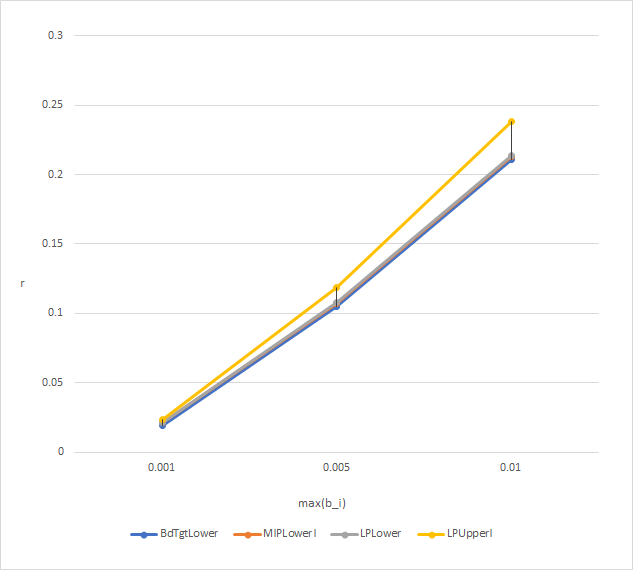
\includegraphics[scale=0.45]{Figures/Case5}
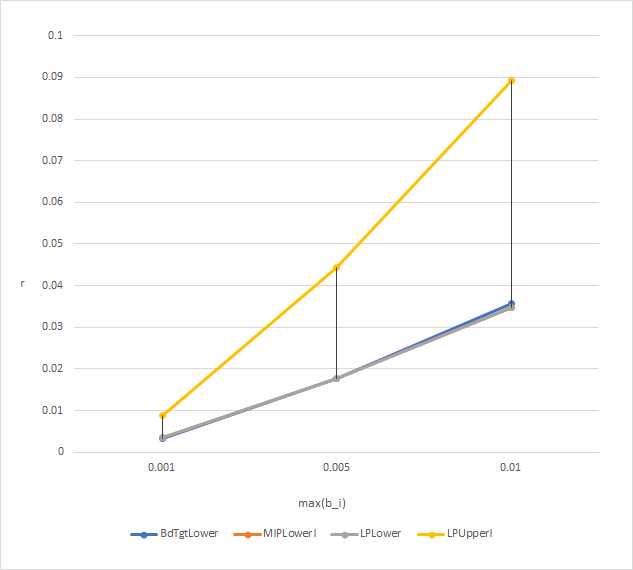
\includegraphics[scale=0.45]{Figures/Case9} \\
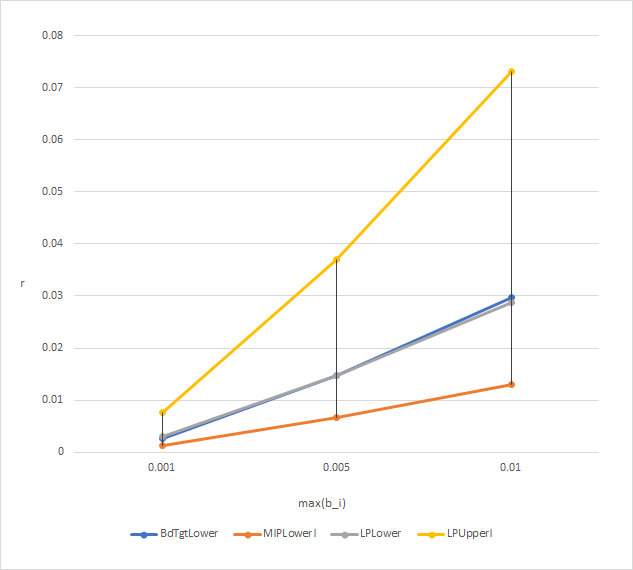
\includegraphics[scale=0.45]{Figures/Case14}
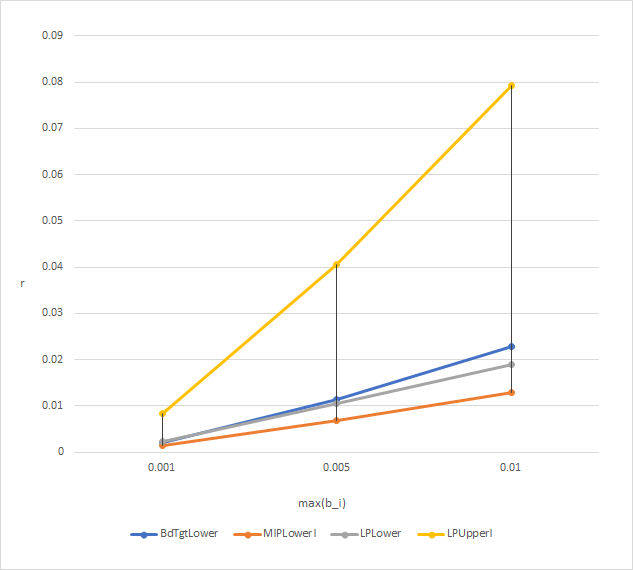
\includegraphics[scale=0.45]{Figures/Case30}
\caption{Case 5 (Top Left), Case 9 (Top Right), Case 14 (Bottom Left), Case 30 (Bottom Right)} \ \\
\end{center}
\label{fig:Graphs1}
\end{figure} 

%\begin{table}[h]
%\begin{center}
%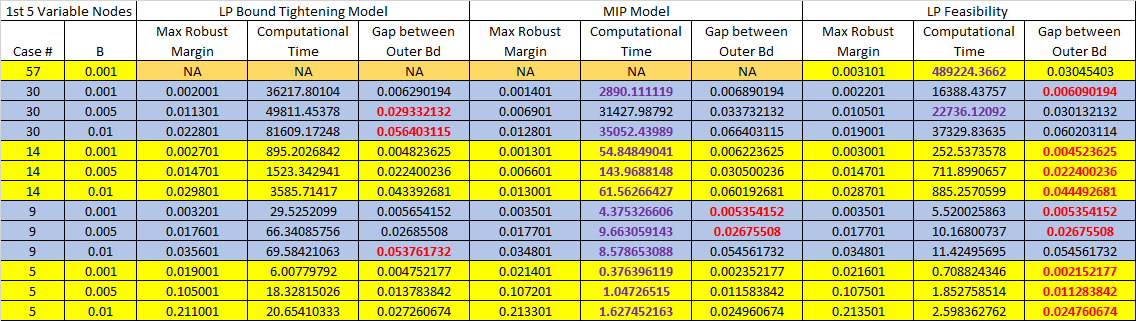
\includegraphics[scale=0.6]{Figures/InnerBoundTable}
%\caption{Robustness Margins for inner bound models } 
%\vspace{0.2in}
%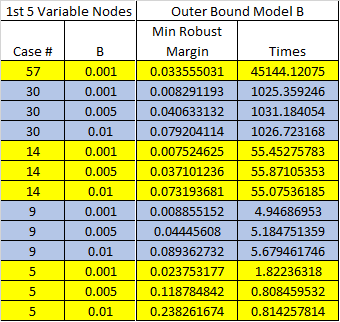
\includegraphics[scale=0.5]{Figures/OuterBoundTable}
%\caption{Robustness Margins for outer bound models}
%\end{center}
%\label{tbl:Table1}
%\end{table} 

As evident from Table 1 we have that the bound tightening model produces a better approximation of the inner bound on the robustness margin as the complexity of the data set increases. 
Certainly one would expect the bound tightening model to out perform the other inner bound models for all cases, but the choice of model parameters has a big effect on the efficiency of the model. 
For instance, setting a low tolerance for a minimal sufficient change in the dimensions of $\bold b$ will cause in most cases an extremely long running time. 
Thus in the lower complexity cases it should be expected that the other models will out perform the bound tightening model as these manually set model parameters will have more of an impact on performance. 
Of special interest is the difference in performance of the MIP and Feasibility inner bound models as the complexity of the data increases. 
In particular it was surprising that the Feasibility model was the only inner bound model capable of efficiently computing the robustness margin for case 57 (see tables 2 and 3). 

\section{Conclusion}

In this paper we have proposed novel and efficient techniques for determining robust solvability of quadratic systems with uncertainty. 
It is worth mentioning that the same machinery can be used to determine robustness margins of solutions to static systems by taking $A$ to be the identity, $e_i=0 \ \forall i$ and simply adjusting $\bold b$ accordingly. 
The models presented here are in some sense just the tip of the iceberg. 
More efficient models can certainly be derived using the theory contained here. 
We present these models only as examples of how efficient algorithms could be constructed utilizing the theoretical results we presented. 

\bibliography{Ref}

\end{document}
